%mark = star, diamond, square, otimes
%\documentclass{article}
%\usepackage{pgfplots}
%\usepackage[justification=centering]{caption}
%\pgfplotsset{compat=newest}
%\begin{document}
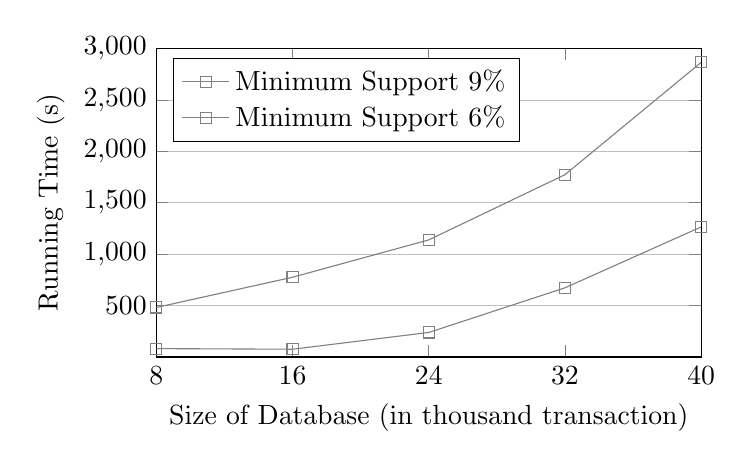
\begin{tikzpicture}
\begin{axis}[
    width=8.5cm,
    height=5.5cm,
    xlabel={Size of Database (in thousand transaction)},
    ylabel={Running Time (s)},
    xmin=8, xmax=40,
    ymin=0, ymax=3000,
    xtick={8,16,24,32,40},
    ytick={500,1000,1500,2000,2500,3000},
    legend pos=north west,
    ymajorgrids=true,
    grid style={line width=.2pt,draw=gray!50},
]
 
\addplot[
    solid,color=gray, every mark/.append style={solid, fill=gray}, mark=square
    ]
    coordinates {
			(8,482)
			(16,776)
			(24,1139)
			(32,1773)
			(40,2865)

	};
    \addlegendentry{Minimum Support 9\%}

\addplot[
    solid,color=gray, every mark/.append style={solid, fill=gray}, mark=square
    ]
    coordinates {
			(8,82)
			(16,76)
			(24,239)
			(32,673)
			(40,1265)

	};
    \addlegendentry{Minimum Support 6\%}

\end{axis}
\end{tikzpicture}
%\end{document}